\documentclass[10pt, titlepage, oneside, a4paper]{article}
\usepackage{array}
\usepackage{caption}
\usepackage{fancyhdr}
\usepackage{graphicx}
\usepackage{hyperref}
\usepackage{indentfirst}
\usepackage{lastpage}
\usepackage{lmodern}
\usepackage[utf8]{inputenc}
\usepackage{polski}

\usepackage{textcomp}

\graphicspath{ {./images/} }
\urlstyle{same}

\title{Specyfikacja Projektu ,,Expert4Home''}
\author{K. Dąbrowski, J. Grygiel, S. Kalisz\\
K. Malinowski, P. Piętka, B.Zdrojewski}
\date{Wersja 1.0\\\today}

\pagestyle{fancy}
\fancyhf{}
\lhead{Specyfikacja Projektu ,,Expert4Home''}
\rhead{Wersja 1.0}
\rfoot{\thepage \hspace{1pt} / \pageref{LastPage}}

\begin{document}

	\maketitle
	\thispagestyle{empty}  
	\newpage
  
	\section{Wstęp} 
  
	\subsection{Cel dokumentu}
	Celem dokumentu jest klarowne przekazanie propozycji realizacji celu projektu. W dokumencie zaprezentowano podstawy \textbf{architektury systemu}, które będą rozwijane i uszczegóławiane wraz z postępem projektu, schematy elementów \textbf{interfejsu użytkownika}, niezbędnych do realizacji kluczowych funkcji systemu, sugerowane \textbf{technologie}, które, na stan wiedzy autorów, wydają się być najlepiej dopasowane do skali i celów projektu, oraz \textbf{metody organizacji pracy}, wraz z \textbf{harmonogramem prac}, które mają zapewnić, że projekt zostanie ukończony w wyznaczonych ramach czasowych.
  
	\subsection{Cel projektu}
	Celem projektu jest zaprojektowanie i zaimplementowanie aplikacji webowej, której przeznaczeniem będzie łączenie specjalistów z danej branży z potencjalnymi klientami. 
	
	Z punktu widzenia specjalisty, aplikacja będzie pozwalać na publikację profilu dowolnej działalności, opartej o realizację usług lub zleceń, oraz zapewniać platformę do kontaktu z klientami.
	
	Natomiast z punktu widzenia klienta, aplikacja będzie pozwalać na wyszukanie specjalisty, skontaktowanie się z nim, ustalenie szczegółów usługi lub zlecenia, a ostatecznie na wyrażenie opinii na temat jakości wykonanej przez niego usługi lub zlecenia.
  
	\subsection{Użytkownicy końcowi}
	Użytkownikami końcowymi mogą być zarówno specjaliści, którzy chcą poszerzyć zasięg swojej działalności lub ułatwić komunikację na linii przedsiębiorca-klient, jak i dowolne osoby poszukujące sprawdzonych i dostosowanych do ich potrzeb usługodawców i zleceniobiorców.
	\newpage  
  
	\section{Architektura systemu}
  
  \subsection{Aktorzy}
	Osoby korzystające z aplikacji będą mogły grać rolę różnych aktorów podczas interakcji z systemem w zależności od celu, który chcą osiągnąć.
	Oznacza to, że ta sama osoba może raz wystąpić w roli eksperta oferującego swoje usługi, a innym razem skorzystać z systemu jako klient szukający wykonawcy zlecenia.

	\subsubsection*{Lista przewidzianych aktorów}
	\begin{itemize}
		\item Ekspert -- Osoba posiadająca wiedzę i umiejętności w danej dziedzinie pozwalające na świadczenie usług innym,
		\item Klient -- Osoba szukająca wykonawcy usług
		\item Stały klient -- Klient, który nawiązał wielokrotną współpracę z \textbf{konkretnym ekspertem}. Ma on dostęp do dodatkowych benefitów udzielonych przez eksperta
		\item Administrator -- Osoba mająca dodatkowe uprawnienia dzięki którym może wypływać na działanie systemu dla zwykłych użytkowników
	\end{itemize}
	
  \subsection{Przypadki użycia}
  Diagram przypadków użycia przedstawia rysunek \ref{fig:ucDiagram}.

  \begin{figure}[h]
	  \centering
	  \includegraphics[width=\textwidth{}]{use_case_diagram.png}
	  \caption{Diagram przypadków użycia}
	  \label{fig:ucDiagram}
  \end{figure}
	\newpage  
  
  \subsection{Diagramy sekwencji}
	Dynamikę działania poszczególnych przypadków użycia przedstawiają poniższe diagramy sekwencji.

	\begin{figure}[!htbp]
		\centering
		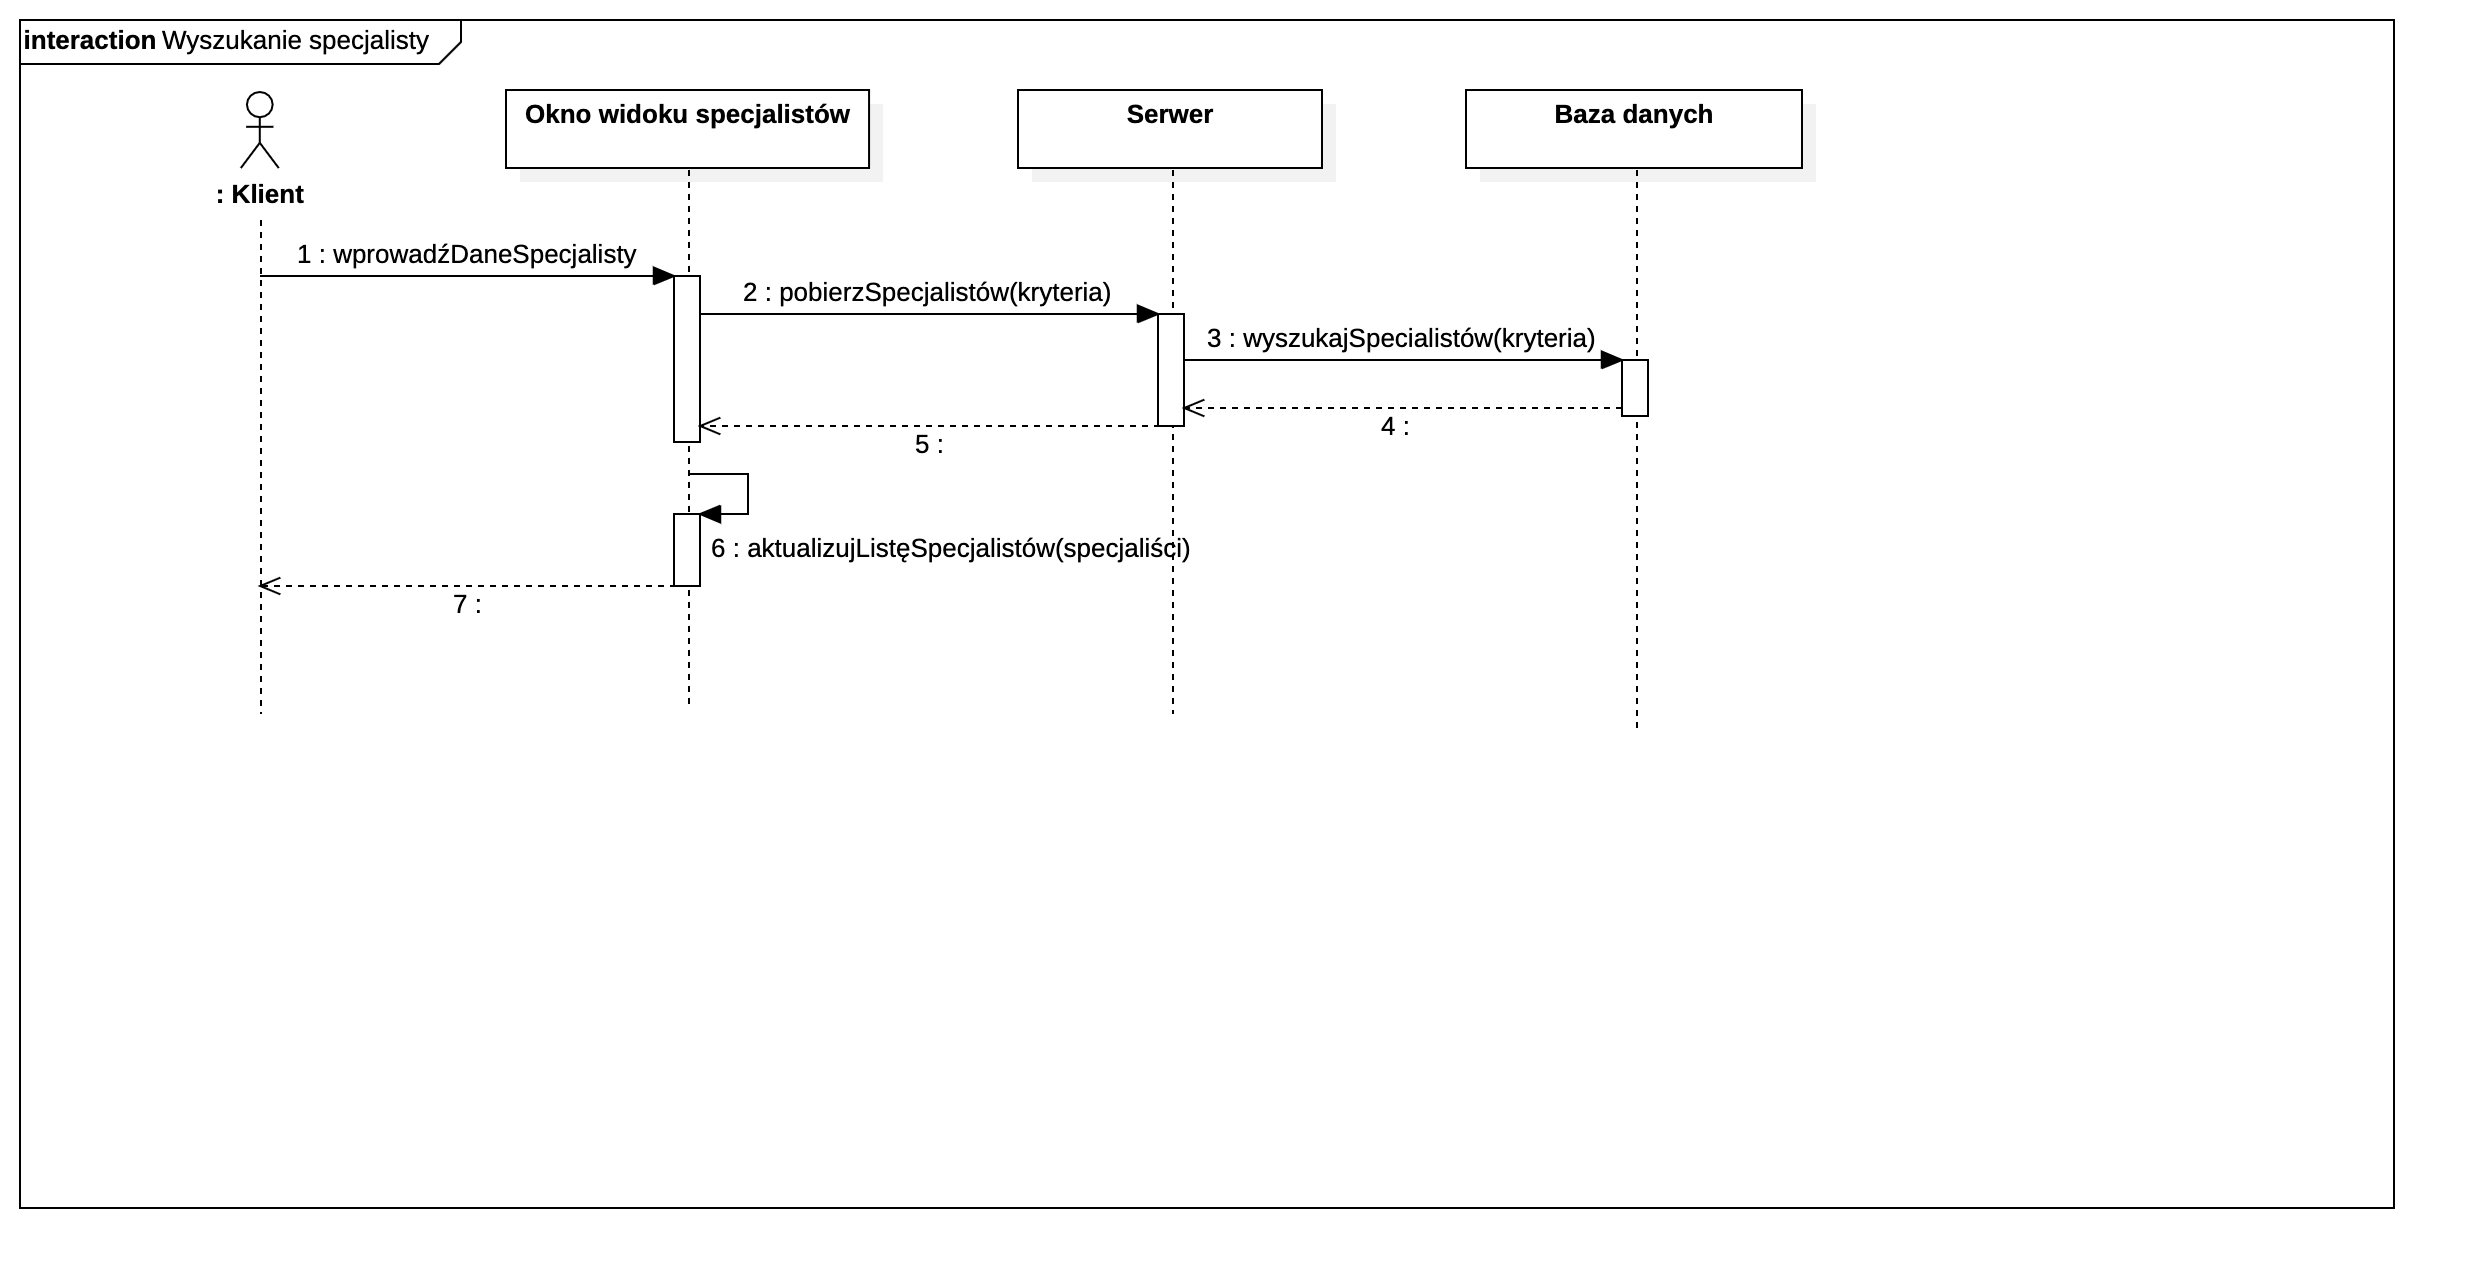
\includegraphics[width=\textwidth{}]{Wyszukanie_specjalisty.png}
		\caption{Wyszukanie specjalisty}
		\label{fig:sequenceDiagramSearchForExpert}
	\end{figure}

	\begin{figure}[!htbp]
		\centering
		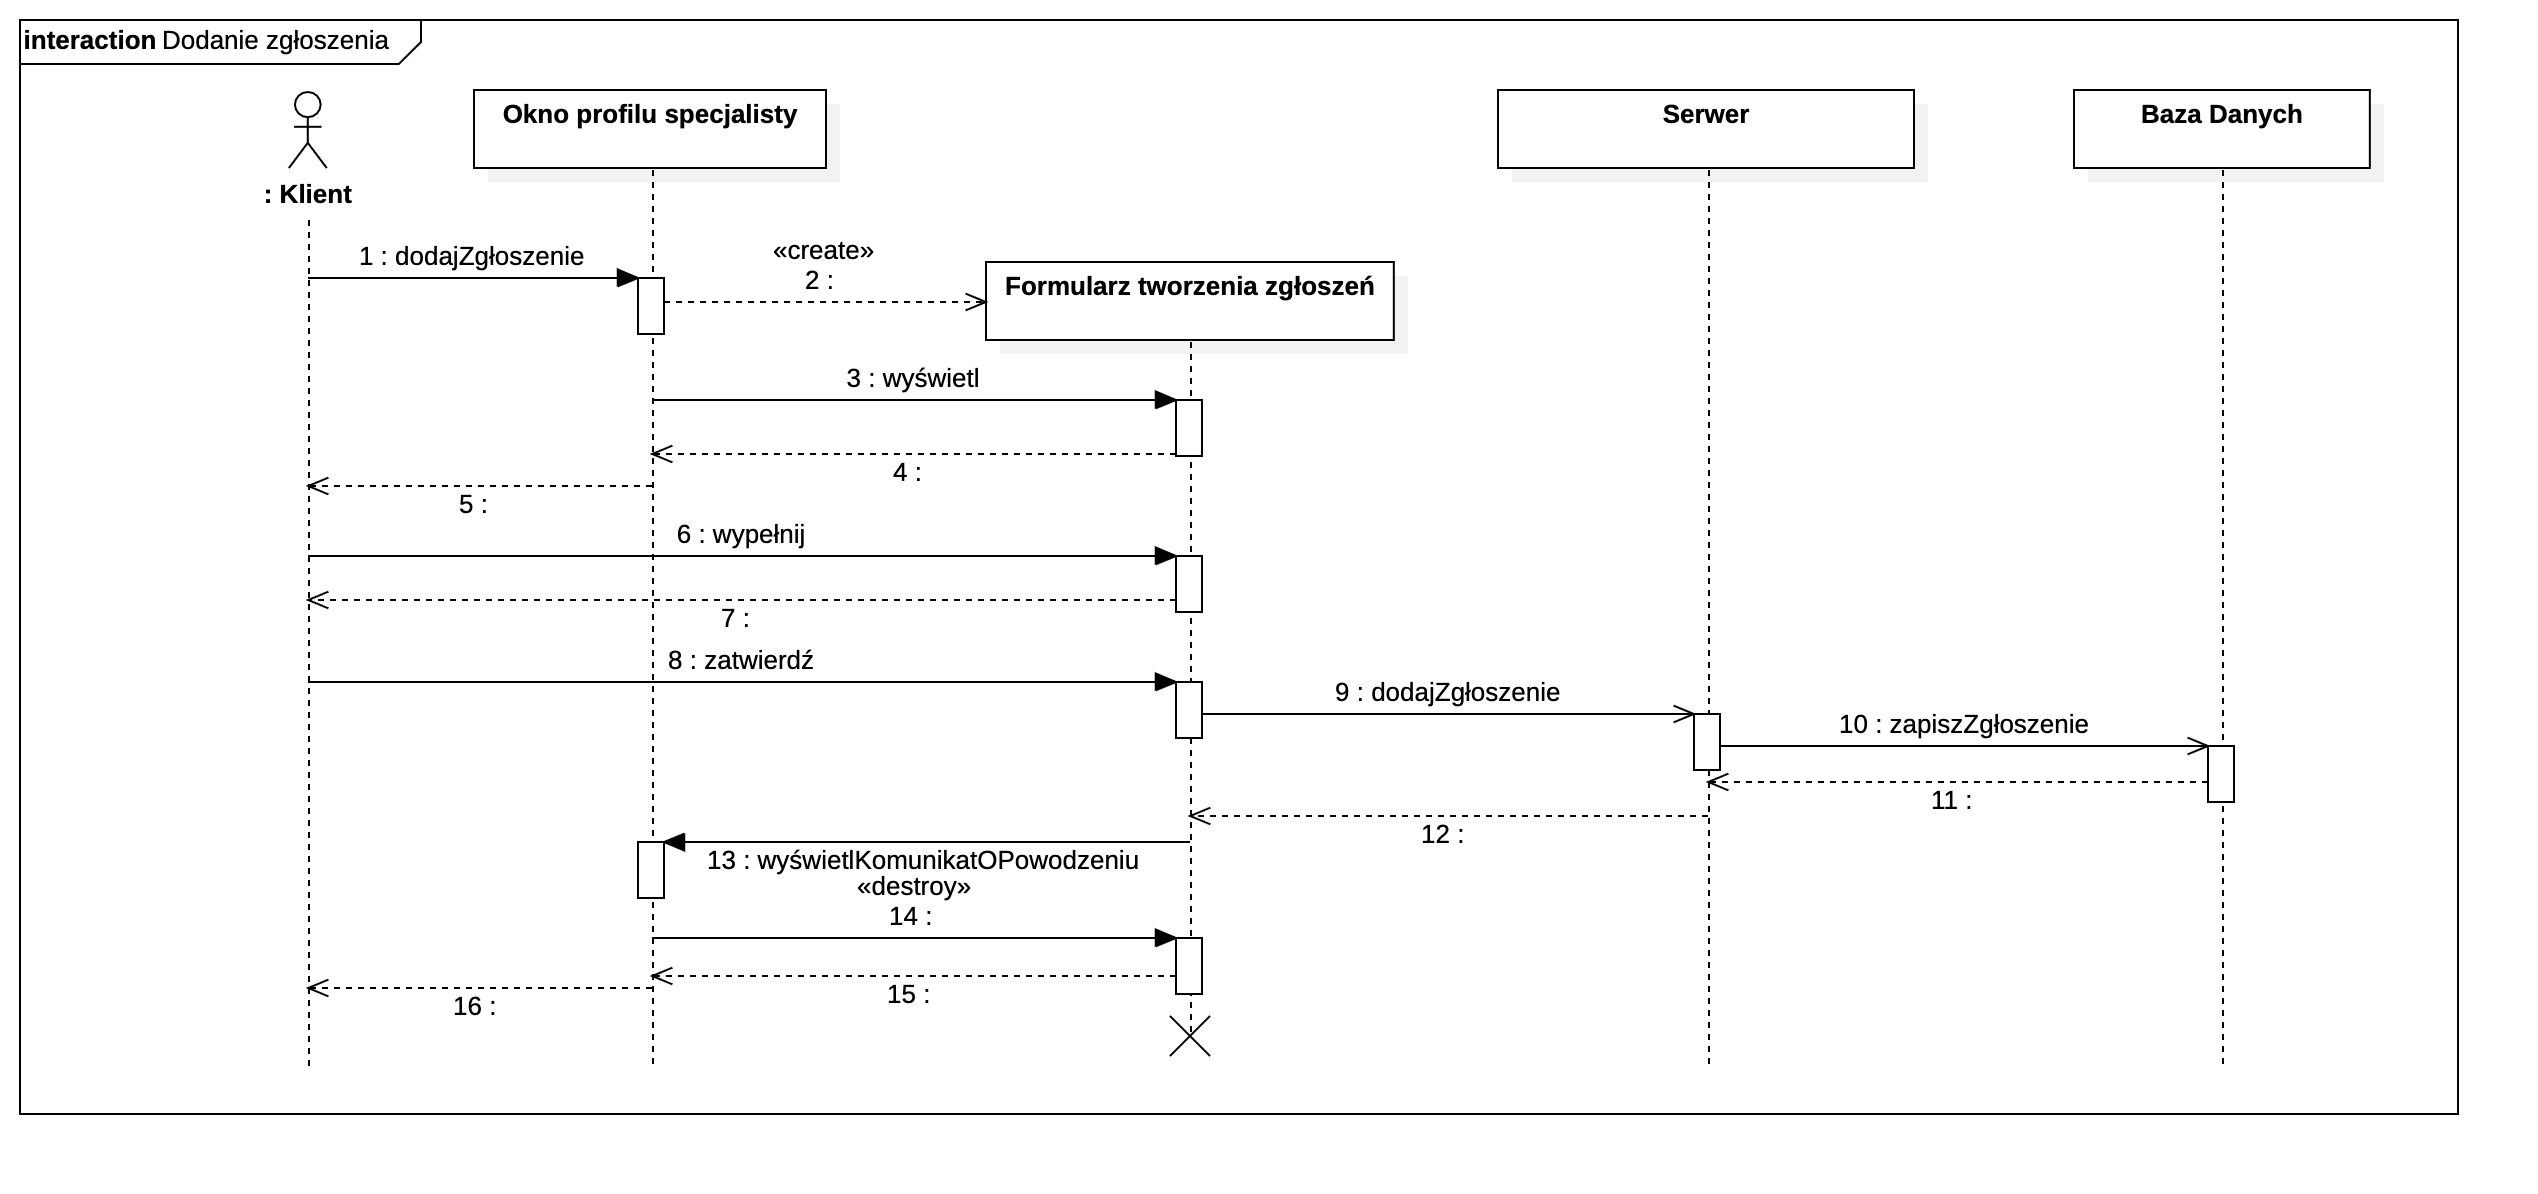
\includegraphics[width=\textwidth{}]{Dodanie_zgloszenia.png}
		\caption{Dodanie zgłoszenia}
		\label{fig:sequenceDiagramAddRequest}
	\end{figure}

	\begin{figure}[!htbp]
		\centering
		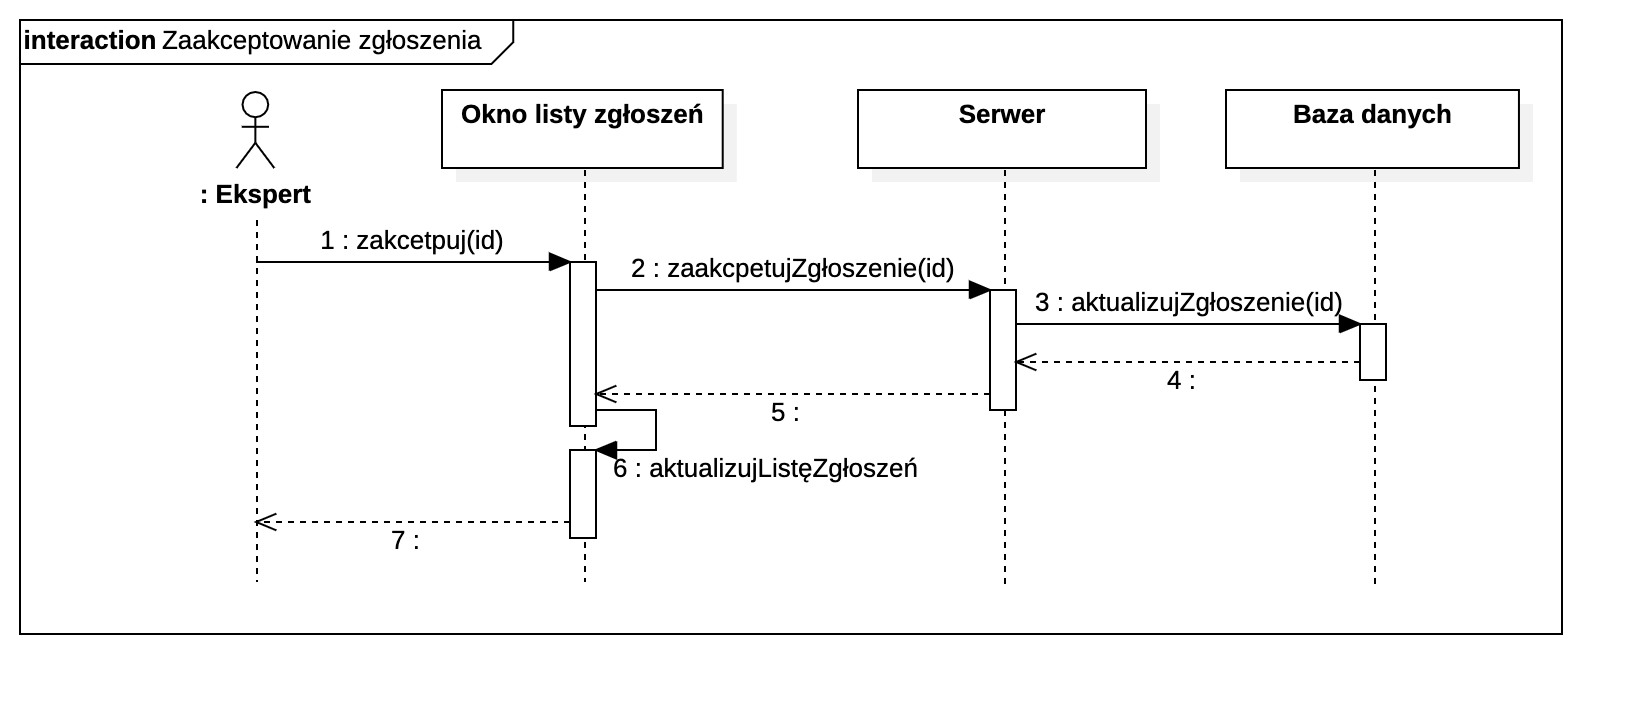
\includegraphics[width=\textwidth{}]{Zaakceptowanie_zgloszenia.png}
		\caption{Zaakceptowanie zgłoszenia}
		\label{fig:sequenceDiagramAcceptRequest}
	\end{figure}

	\begin{figure}[!htbp]
		\centering
		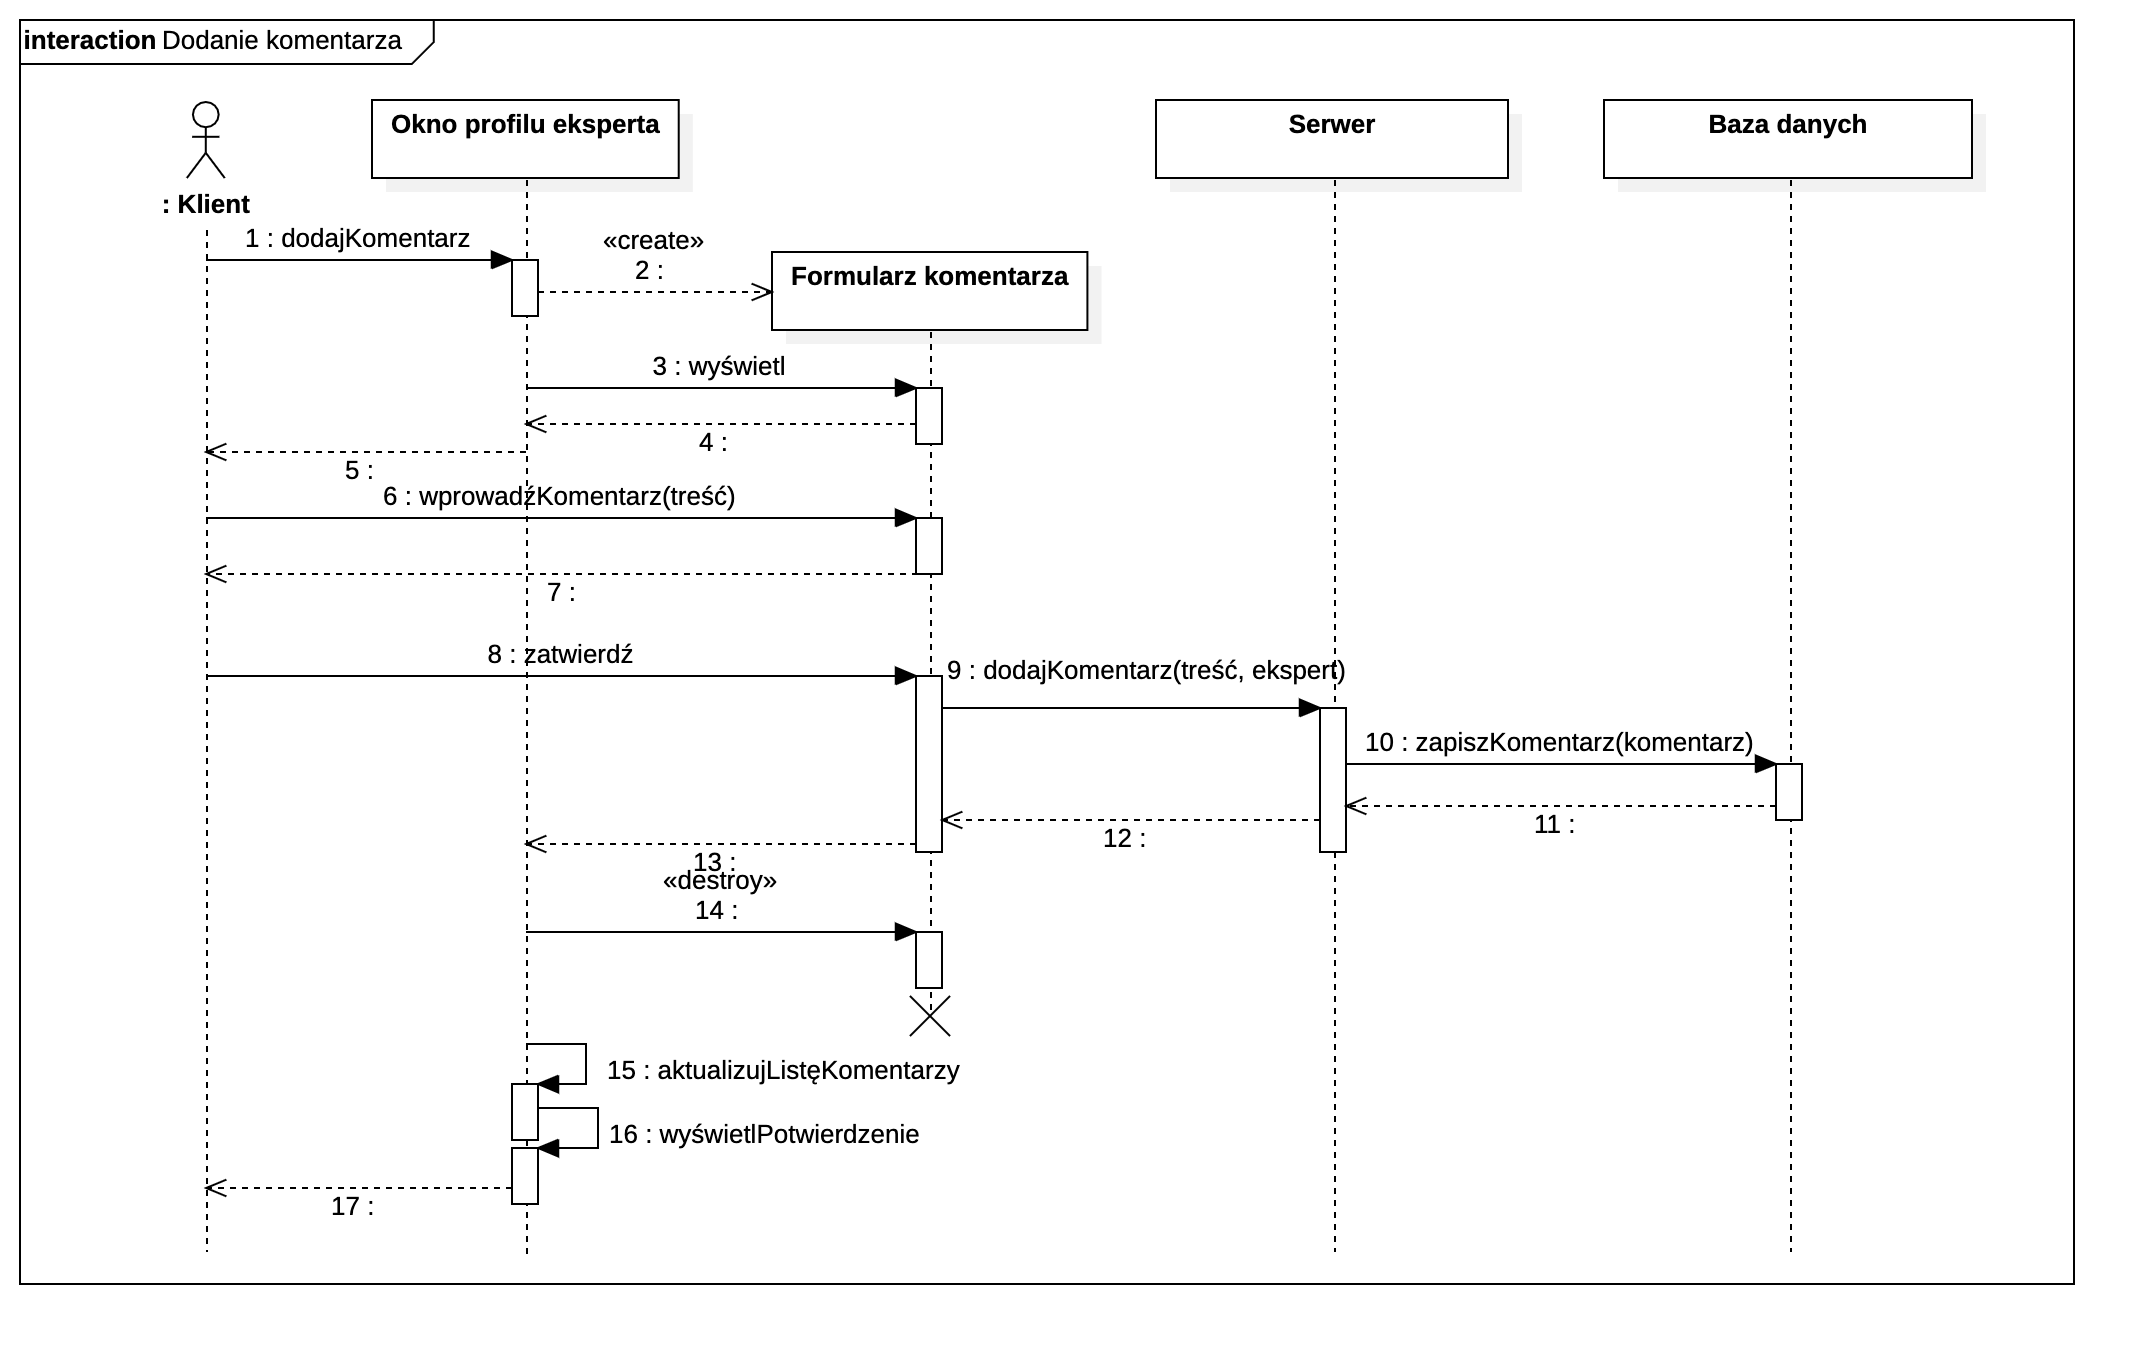
\includegraphics[width=\textwidth{}]{Dodanie_komentarza.png}
		\caption{Dodanie komentarza}
		\label{fig:sequenceDiagramAddComment}
	\end{figure}
	\newpage  
  
	\section{Interfejs użytkownika}
  
	\subsection{Ekran główny}
	\begin{figure}[!htbp]
  \begin{center}
  {%
		\setlength{\fboxsep}{0.5pt}%
		\setlength{\fboxrule}{0.5pt}%
		\fbox{
			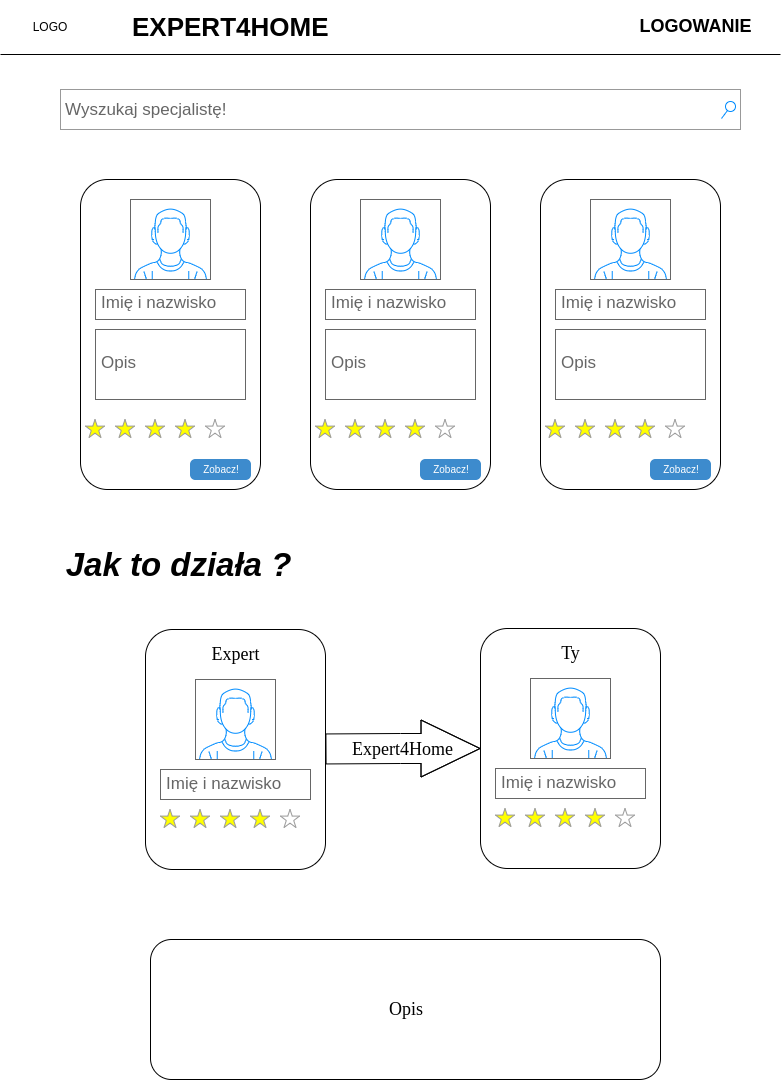
\includegraphics[width=\textwidth]{home_view.png}
		}%
	}%
  \captionof{figure}{Schemat ekranu głównego}
  \end{center}
  \end{figure}
	\newpage

	\subsection{Ekran wyszukiwania specjalisty}
	\begin{figure}[!htbp]
  \begin{center}
  {%
		\setlength{\fboxsep}{0.5pt}%
		\setlength{\fboxrule}{0.5pt}%
		\fbox{
			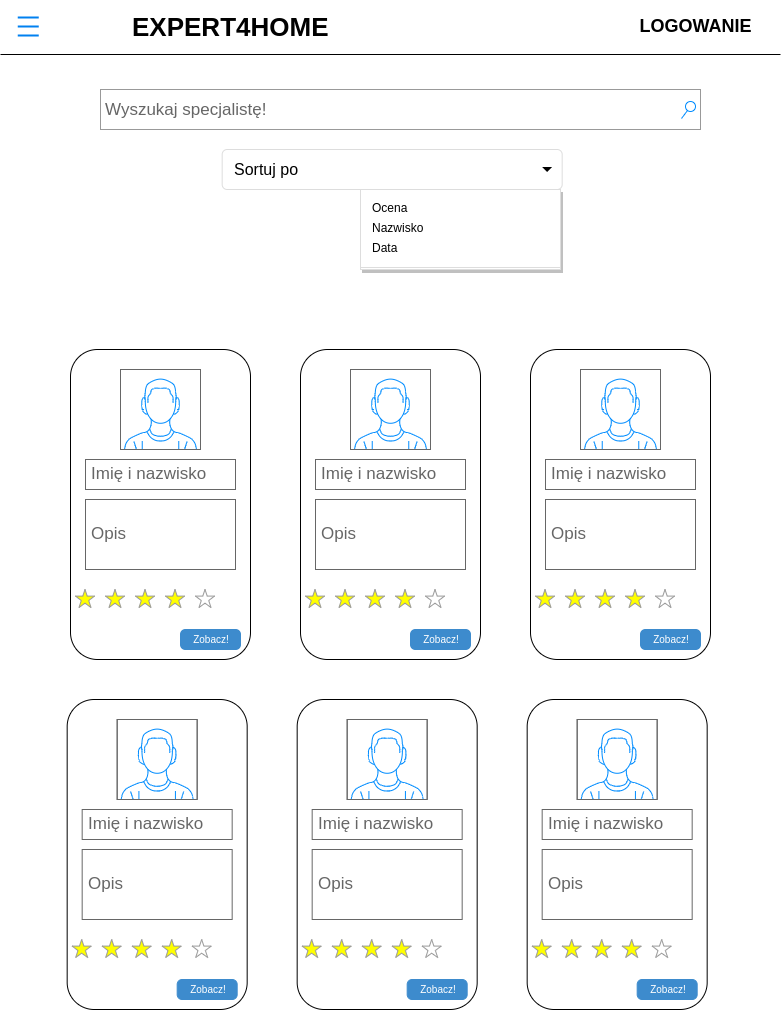
\includegraphics[width=\textwidth]{search_expert_view.png}
		}%
	}%
  \captionof{figure}{Schemat ekranu wyszukiwania specjalisty}
  \end{center}
  \end{figure}
	\newpage

	\subsection{Ekran profilu specjalisty}	
	\begin{figure}[!htbp]
  \begin{center}
  {%
		\setlength{\fboxsep}{0.5pt}%
		\setlength{\fboxrule}{0.5pt}%
		\fbox{
			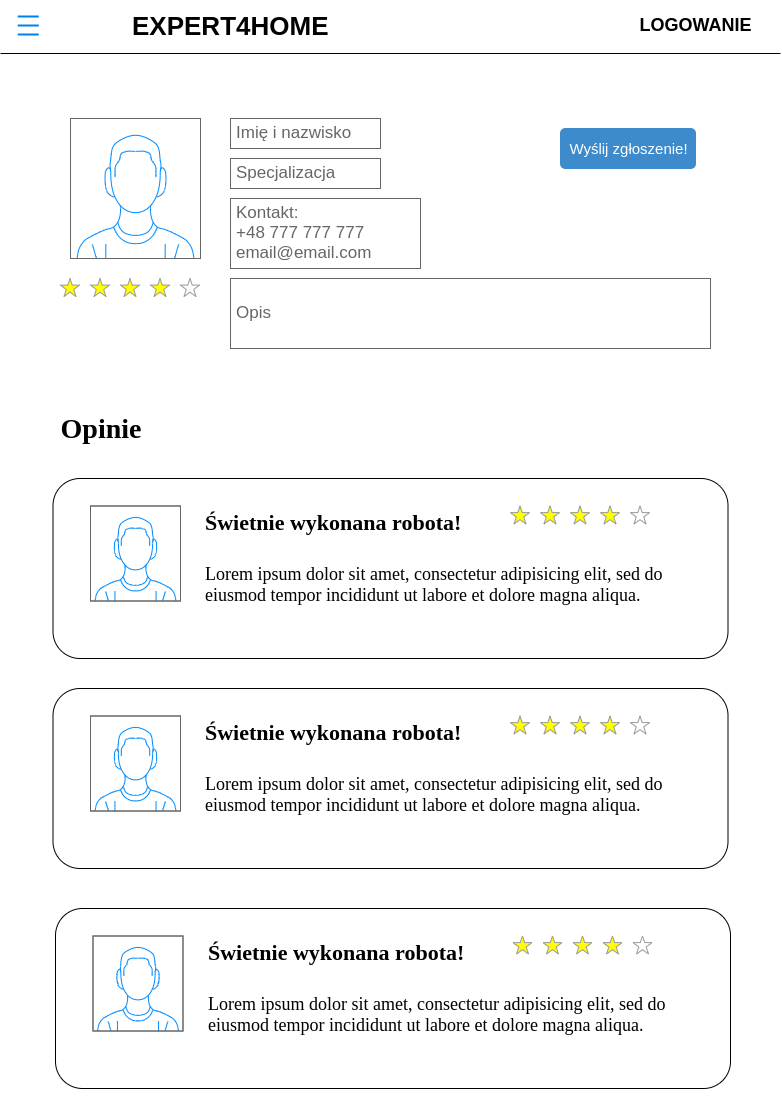
\includegraphics[width=\textwidth]{expert_profile_view.png}
		}%
	}%
  \captionof{figure}{Schemat ekranu profilu specjalisty}
  \end{center}
  \end{figure}
	\newpage
	
	\subsection{Dialog zgłoszenia}	
	\begin{figure}[!htbp]
  \begin{center}
  {%
		\setlength{\fboxsep}{0.5pt}%
		\setlength{\fboxrule}{0.5pt}%
		\fbox{
			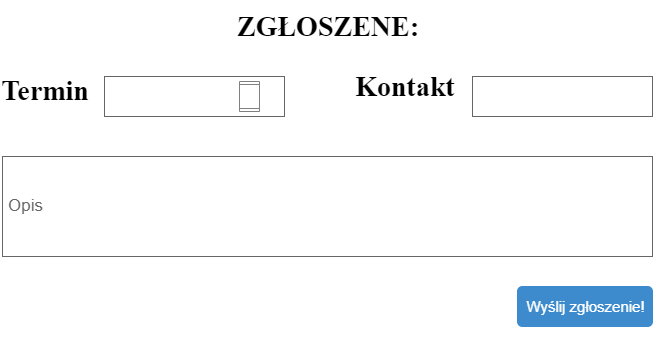
\includegraphics[width=\textwidth]{client_report.png}
		}%
	}%
  \captionof{figure}{Schemat dialogu zgłoszenia}
  \end{center}
  \end{figure}
	\newpage
	
	\subsection{Ekran zgłoszeń klienta}
	\begin{figure}[!htbp]
  \begin{center}
  {%
		\setlength{\fboxsep}{0.5pt}%
		\setlength{\fboxrule}{0.5pt}%
		\fbox{
			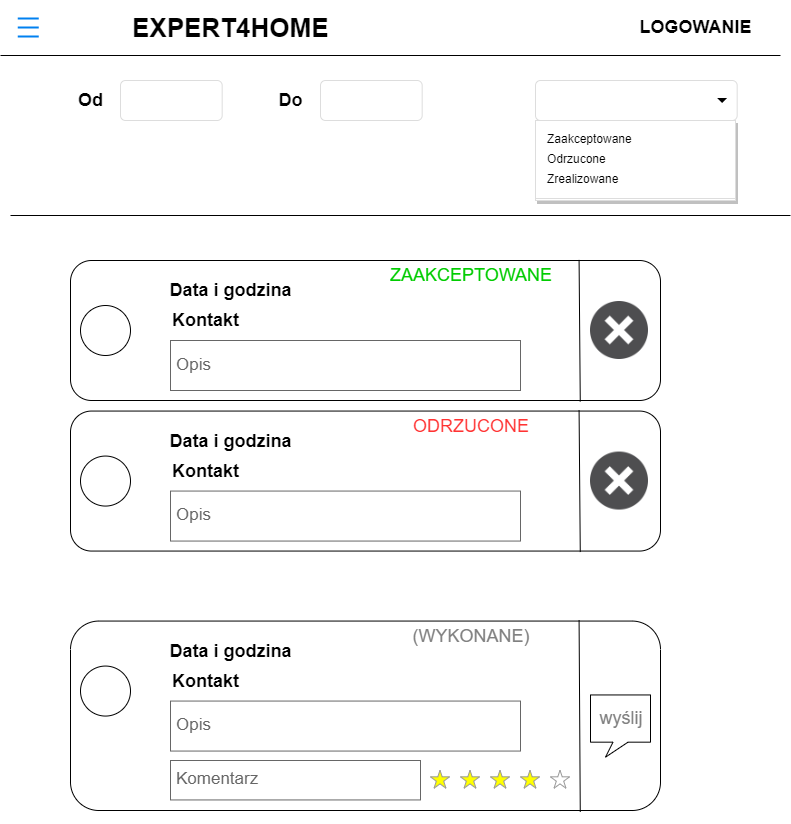
\includegraphics[width=\textwidth]{client_my_reports.png}
		}%
	}%
  \captionof{figure}{Schemat ekranu zgłoszenia klienta}
  \end{center}
  \end{figure}
	\newpage
	
	\subsection{Ekran zgłoszeń specjalisty}
	\begin{figure}[!htbp]
  \begin{center}
  {%
		\setlength{\fboxsep}{0.5pt}%
		\setlength{\fboxrule}{0.5pt}%
		\fbox{
			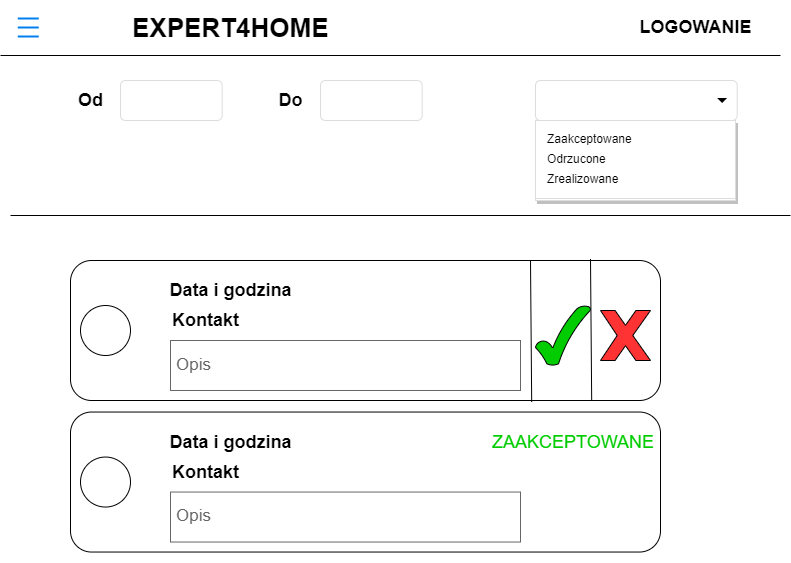
\includegraphics[width=\textwidth]{expert_my_reports.png}
		}%
	}%
  \captionof{figure}{Schemat ekranu zgłoszenia specjalisty}
  \end{center}
  \end{figure}
	\newpage 
  
	\section{Szczegóły implementacji}  
  
	\subsection{Środowisko deweloperskie}  
	Jednym z ważniejszych wyzwań jest zapewnienie spójności środowisk pomiędzy uczestnikami zespołu. Wszelkie nawet najmniejsze odchylenia mogą prowadzić do błędów, co gorsza większość problemów może być nie możliwa do odtworzenia na innych maszynach. Ponieważ wybraliśmy Javę 8 jako język programowania niezbędna jest automatyzacja budowania oraz zarządzania zależnościami itp.
	
	Postanowiliśmy użyć programu Gradle, posiada on prostą i przejrzystą składnie ułatwiającą pracę. Mimo ułatwienia jakim jest Gradle, nie jest wystarczającym środkiem zapewnienia spójności. W celu osiągnięcia jej postanowiliśmy skorzystać z kontenerów Dockerowych. Ze względu na rozmiar kontenerów Windowsowych, jedyną możliwą opcją są kontenery Linuxowe. Oznacza to iż platformą docelową dla każdego fragmentu aplikacji jest Alpine Linux. Konteneryzacja aplikacji ułatwia również późniejsze uruchomienie jej w środowisku chmurowym. Każdy z 3 najpopularniejszych dostawców oferuje hosting dla kontenerów.
  
	\subsection{Zastosowane technologie}

	\subsubsection{Front-end}
	Do stworzenia front-endu aplikacji postanowiliśmy wykorzystać bibliotekę React.js języka JavaScript. Jest to najbardziej popularna biblioteka front-end którą rozwija Facebook. Pozwala ona na napisanie front-endu jako SPA - Single Page Application. Wybraliśmy tą bibliotekę ponieważ:
	\begin{itemize}
	\item jest ona najbardziej popularna,
	\item jest wygodna w stosowaniu przy małych aplikacjach (w przeciwieństwie do Angulara),
	\item jest oparta na komponentach,
	\item ułatwia tworzenie interaktywnych UI.
	\end{itemize}
	
	Do stworzenia aplikacji skorzystamy z metody create-react app która pozwala na stworzenie aplikacji bez konieczności dużej ilości konfiguracji. Do stylowania projektu zostanie użyte scss modules oraz styled components. Do zarządznia stanem aplikacji zostanie użyty Redux. Do nawigowania między podstronami zostanie użyty react-router.
	
	\subsubsection{Back-end}	
	Do serwerowej części projektu postanowiliśmy wykorzystać kilka technologii. Zostaną one opisane poniżej.
	
	\paragraph{SpringBoot} \mbox{} \par
	Do napisania kodu części serwerowej aplikacji wybraliśmy framework SpringBoot języka Java.
	Jest to rozwiązanie sprawdzone przez wiele firm i rozwijane oraz wspierane już przez wiele lat. Dzięki temu możemy korzystać z dopracowanych bibliotek oraz zdobyć cenne doświadczenie.

	SpringBoot jest bazowany na frameworku Spring jednak w przeciwieństwie do niego znacznie ogranicza niepotrzebną konfigurację na rzecz konwencji.
	Dzięki takiemu podejściu programista może skupić się na realizowaniu funkcjonalności zamiast na przygotowywaniu środowiska.

	\paragraph{Tomcat} \mbox{} \par
	Do uruchomienia aplikacji oraz obsługi połączeń sieciowych zastosowany został serwer Tomcat.
	Jest to rozwiązanie o otwartym kodzie źródłowym wspierane przez organizację Apache.
	Stanowi domyślne rozwiązanie dla aplikacji sieciowych pisanych w języku Java.

	\paragraph{MySQL} \mbox{} \par
	Do przechowywania danych biznesowych aplikacji wybraliśmy bazę MySQL.
	Ponieważ dane maja wyraźną strukturę uznaliśmy, że rozwiązanie oparte na SQL będzie dobrze rozwiązywało problemy związane ze składowaniem danych.
	Baza MySQL posiada otwarty kod źródłowy, ma zaimplementowane wszystkie najważniejsze funkcjonalności silników bazodanowych takie jak transakcje, widoki czy wyzwalacze i jest to szeroko używane i sprawdzone rozwiązanie.

	\paragraph{Nginx} \mbox{} \par
	Przez wiele lat dominującym serwerem http na rynku był Apache. W 2019 został on zdetronizowany przez Nginxa. 
	Zdecydowaliśmy się użyć nowego króla. Głównych jego cechą jest możliwość obsługiwania bardzo dużej liczby
	połączeń jednocześnie, dzięki asynchronicznemu podejściu do obsługi zapytań. Apache obsługuje połączenia
	synchronicznie, tj. tworzy nowy proces dla każdego połączenia. Ponad to składnia konfiguracji Nginx jest
	znacznie bardziej przejrzysta niż konfiguracja Apache. Dodatkową zaletą Nginxa jest jego popularność. Oznacza
	to iż w sytuacji natrafienia na trudności istnieje duża szansa iż ktoś już kiedyś natrafił na podobny problem.
	
	\subsubsection{Kontrola wersji}
	W celu zapewnienia możliwości monitorowania i wycofywania zmian w kodzie źródłowym aplikacji oraz równoległej, bezkonfliktowej pracy wszystkich członków zespołu, postanowiono skorzystać z systemu kontroli wersji. Wybrano znany i szeroko stosowany system \textbf{git}. Dodatkowo, w celu zapewnienia łatwego dostępu do repozytorium aplikacji, postanowiono skorzystać z serwisu \textbf{Github}.
	
	Repozytorium składać się będzie z co najmniej dwóch gałęzi: \textit{master} i \textit{development}. Na gałęzi \textit{development} będą prowadzone prace deweloperskie. Wszelkie dodatkowe gałęzie, które zostaną stworzone na potrzeby konkretnych funkcjonalności, będą łączone właśnie z tą gałęzią.
	
	Gdy wszystkie zmiany na gałęzi \textit{development} zostaną przetestowane i stabilność danej wersji aplikacji zostanie potwierdzona, zostaną one połączone z gałęzią \textit{master}.
	  
	\subsubsection{Wdrożenie oprogramowania}
	Istnienie kontenerów Dockerowy otwiera przed naszym zespołem wiele nowych możliwości. Dzięki sposobowi dystrybucji jakim jest Docker Hub w bardzo prosty sposób można uzyskać dostęp do wielu już stworzonych obrazów dysków. Możliwym jest również rozstawienie własnego rejestru obrazów. W efekcie pobieranie wszelkiego rodzaju zależności sprowadza się do jednej komendy, gdzie każda zależności "myśli" że jest oddzielnym systemem operacyjnym. Przykładowo, jeżeli potrzebujemy bazy postgreSQL wystarczy wywołać komendę \texttt{docker pull postgres}, odpowiedni obraz zostanie pobrany.
	
	Docelowo środowiskiem produkcyjnym aplikacji będzie chmura Microsoft Azure. Dokładnie oferowany przez MSA hosting kontenerów. Zdecydowaliśmy się na Azure ze względu na możliwość połączenia ponieważ korzystamy z pakietu Azure DevOps. Azure Devops pozwala na zarządzanie zadaniami, hostowanie prywatnych rejestrów Dockerowych oraz co najważniejsze, pozwala na definiowanie procesów CI/CD. W odpowiednim etapie dojrzałości projektu planujemy skorzystać z właśnie tej funkcjonalności w celu usprawnienia całego procesu wytwarzania oprogramowania.
	  
	\subsection{Plan testów}	
	Ponieważ w projekcie ma być używana metodyka SCRUM, korzystanie z techniki TDD nie jest obowiązkowe. Mimo to  testy jednostkowe nadal okazują się przydatne. Pozwalają na pewnego rodzaju dokumentowanie kodu za pomocą testów, pozwalają zrozumieć celowość przykładowej metody, sposób wywoływania i jak działa bez wnikania w szczegóły kodu. Może to się okazać przydatne/kluczowe, gdy piszemy kod do jeszcze nieistniejącej klasy, metody lub funkcjonalności, a więc ułatwia w znaczący sposób zrównoleglenie pracy nad problemem. Testy jednostkowe zazwyczaj odnoszą się do klasy, lub metody, pokrywają możliwe scenariusze i sprawdzają czy metoda/klasa dobrze je obsłużyła. W razie gdy metoda polega na innej klasie, niż do tej, do której należy, stosuje się atrapę obiektu/ów (mock), która symuluje przy wywołaniu metody zwrócenie wartości, jaką mogłaby zwrócić prawdziwa funkcja. Testy jednostkowe narzucają w sposób niebezpośredni takiego pisania kodu, by ograniczyć te zależności, co jest zresztą dobrą praktyką. Testy integracyjne pozwalają już sprawdzić z zależnościami czy wszystko wypada dobrze. Może mieć wiele potencjalnych punktów awarii, a nawet być zależny od konfiguracji. Dlatego są równie ważne. Dobre pokrycie kodu testami jednostkowymi jest w stanie przyspieszyć znalezienie błędu w testach integracyjnych. Jak widać, pisanie testów jest opłacalne, mimo tego, że nakłada pisania więcej kodu.
	\newpage 
 
	\section{Szczegóły organizacji pracy}  
 
	\subsection{Harmonogram prac}
	\begin{center}
  \begin{tabular}{ | m{3cm} | m{7cm} | } 
  \hline
  Ostateczny termin & Etap projektu \\
  \hline
  20.09.2019 & Utworzenie zespołu \\
	\hline
  30.09.2019 & Przeprowadzenie spotkania organizacyjnego \\  
  \hline
  31.10.2019 & Zaprojektowanie podstawowej wersji projektu \\
  \hline
  17.12.2019 & Zapoznanie się z technologiami wymaganymi do realizacji projektu \\
  \hline
  12.01.2020 & Utworzenie jednolitego środowiska deweloperskiego u wszystkich członków zespołu \\
  \hline
  26.01.2020 & Utworzenie specyfikacji projektu \\
  \hline
  8.03.2020 & Zaimplementowanie podstawowej wersji projektu \\
  \hline
  22.03.2020 & Przeprowadzenie spotkania organizacyjnego \\
  \hline
  12.04.2020 & Zaprojektowanie rozszerzonej wersji projektu \\
  \hline
  31.05.2020 & Zaimplementowanie rozszerzonej wersji projektu \\
  \hline
  14.06.2020 & Uzupełnienie specyfikacji projektu \\
  \hline
  \end{tabular}
  \captionof{table}{Harmonogram prac}
  \label{sophisticatedtable}
  \end{center}
 
	\subsection{Metodyka wytwarzania oprogramowania}
	Dzięki użyciu Azure DevOps mamy dostęp do narzędzi scrumowych oraz tablicy kanban. Wszystko mieści się w ramach tzw. \textit{Boards}. Wymagana funkcjonalność jest zawarta jako \textit{User Stories}, które to oddzielają się na konkretne zadania (\textit{Tasks}).
 
	Tablica kanban przechowuje \textit{User Stories} z następującym przepływem: \textit{TODO} (funkcjonalność, która jest dopiero planowana)\textrightarrow \textit{In progress} (w trakcie wykonywania)\textrightarrow \textit{Resolved} (problem rozwiązany)\textrightarrow \textit{Closed} (rozwiązanie potwierdzone i zamknięte).
 
	Pełna lista \textit{User Stories} znajduje się w \textit{backlogu}.

	Zadania (\textit{Tasks}) są wykonywane w ramach sprintów. Są one podzielone na \textit{User Stories}, które z kolei są rozdzielone na konkretne zadania. Te z kolei mają następujący przepływ: Open\textrightarrow \textit{In Progress} \textrightarrow \textit{Code Review}\textrightarrow \textit{Merge} (testy całości po \textit{merge'u})\textrightarrow \textit{Closed}.
	
	\subsection{Zastosowane narzędzia}
	% todo kd azure devops, slack
	Do zażądania zasobami ludzkimi oraz przepływem pracy zastosujemy odpowiednie narzędzia ułatwiające współpracę nad projektem i komunikację w zespole.

	\paragraph{Azure Devops} \mbox{} \par
	Usługa ta jest jednym z produktów typu ,,software as a service'' dostarczanym przez firmę Microsoft.
	Dzięki współpracy Politechniki z Microsoft mamy darmowy dostęp do narzędzi między innym na zarządzanie projektem w wybranej metodyce. Ułatwia to podział zadań w zespole.

	\paragraph{Slack} \mbox{} \par
	Do komunikacji między członkami zespołu wybraliśmy aplikację Slack. Jest to rozwiązanie z powodzeniem stosowane zarówno w małych firmach jak w światowych korporacjach.
	Umożliwia podział konwersacji na różne kanały. Pozwala również na łatwe wysyłanie wiadomości bezpośrednio do wybranych osób.
	Slack posiada również rozbudowany system rozszerzeń, dzięki temu w razie potrzeb można zwiększyć dostępną funkcjonalność.

	\paragraph{Git} \mbox{} \par
	W celu umożliwienia symultanicznej pracy nad kodem przez różnych członków zespołu korzystamy z Gita jako narzędzi do kontroli wersji.
	Pozwala on na łatwe łączenie pracy wykonanej przez różne osoby oraz oddzielenie pracy nad poszczególnymi funkcjonalnościami do osobnych gałęzi.
	Podczas współpracy kierujemy się wytycznymi \textit{Git Workflow}.
 
\end{document}
